\chapter{ANÁLISIS Y DISCUSIÓN DE RESULTADOS}
En este capítulo, se continuaron las 3 últimas fases de la metodología seleccionada.

\section{Modelamiento}
Antes de crear los modelos correspondientes, y después de definir los valores de entrada y parámetros (las subsecciones que se detallarán a continuación), se asigna una semilla inicial con un valor fijado por el usuario con el fin de evitar resultados aleatorios para futuras iteraciones. Se establece, además, una ruta local en donde se almacena cada punto de control basado en la mejora de la pérdida del subconjunto de validación con respecto a su iteración anterior. En caso de un estancamiento de esta última durante 10 épocas, es decir, si el valor de la pérdida no decrementa, el modelo dejará de entrenar. A esta regla se le añade la reducción de la tasa de aprendizaje luego de 5 épocas en caso el valor de la exactitud del subconjunto de validación no refleje un incremento. El objetivo de estas condiciones es evitar el sobreajuste en los modelos durante el entrenamiento.

Por último, es importante asignar un peso distinto para cada una de las dos clases de la variable dependiente \textit{state}. Con el fin de evitar un mal entrenamiento, los pesos de ambas clases se balancean y se almacenan en un diccionario con su etiqueta correspondiente.

\textbf{Actividad 1: Desarrollar modelo predictivo de Metainformación}
\\
Se diseñó el modelo de descripciones basada en un Perceptrón Multicapa (MLP por sus siglas en inglés) bajo la arquitectura de la Figura \ref{4:fig34} y teniendo como referencia a los autores \citeauthor{pr_yu2018deeplearning}. Se asignaron 100 épocas y el número de lotes fue 32.

\begin{figure}[!ht]
	\begin{center}
		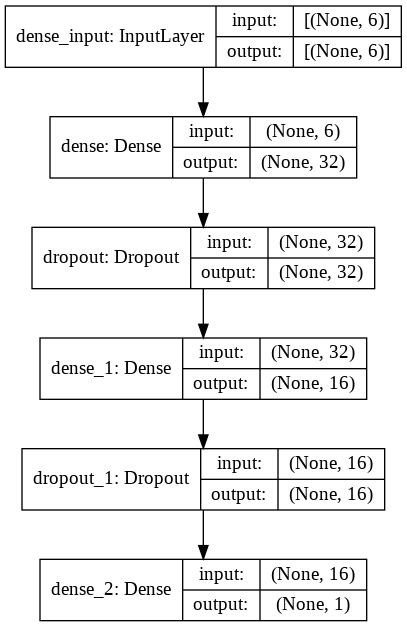
\includegraphics[width=0.40\textwidth]{4/figures/model_mlp_metadata.png}
		\caption[Arquitectura de modelo MLP para la metadata]{Arquitectura de modelo MLP para la metadata.\\
			Fuente: Elaboración propia.}
		\label{4:fig34}
	\end{center}
\end{figure}

La arquitectura comienza con la capa de entrada alimentadas por las 6 variables consideradas, que representan la cantidad de neuronas, tanto de entrada como de salida.

Si bien no existe alguna regla general para definir el número de capas óptimas, así como los hiperparámetros que se deben configurar en ellas, se puede utilizar como referencia algunas metodologías como las Reglas del Pulgar según \cite{tec_ranjan2019thumbrules}.

De acuerdo a una de ellas, el número de capas ocultas comienza con 2 sin contar la última. La primera capa densa continúa a la capa de entrada, mientras que la segunda aparece después de la primera capa de desactivación.

Otro punto considerado fue el número de nodos o neuronas de las capas intermedias. Estas deben seguir una progresión geométrica de 2, donde la primera capa debe ser la mitad del número de variables en la capa de entrada. Dado que la mitad de 6 es un valor que no cumple, un número potencial puede ser 4.

El autor también menciona tener en consideración utilizar la función de activación \textit{\textbf{relu}} para las capas intermedias, una tasa de abandono de por lo menos 0.5 para las capas de desactivación, tamaño de salida de 1 neurona y función de activación \textit{\textbf{sigmoide}} por tratarse de un problema de clasificación binaria, utilizar el optimizador \textit{\textbf{adam}}, comenzar con 20 épocas en adelante de acuerdo al progreso de los resultados y fijar un tamaño de lote bajo progresión geométrica de 2; además de otros requerimientos previamente establecidos como la ponderación de clases para la variable dependiente en caso de datos desbalanceados y escalado de datos antes del entrenamiento.

Estas opciones fueron probadas en el modelo y evaluadas con las métricas correspondientes. Sin embargo, al calibrar el modelo y comparar distintos resultados, se obtuvo que la mejor cantidad de neuronas para la primera capa densa era de 32. De este modo, la siguiente capa intermedia se le asignó la mitad (16). La función de activación \textit{\textbf{tanh}} para la segunda capa oculta presentó mejores resultados, así como tasas de abandono entre 0.25 y 0.3 para las capas de desactivación. El criterio para elegir esta función se explica en el modelo de descripción, en el cual también fue aplicado. Por último, además de \textit{adam}, se realizó experimentos con otros optimizadores como por ejemplo \textit{RMSprop} siendo este el resultado más cercano. Al final, \textit{adam} fue escogido pero con una tasa de aprendizaje baja como 0.005 debido a que el modelo tendía a aprender muy rápido durante el transcurso de las épocas. Al ratio de decaimiento se le asignó, entonces, el valor de 0.00005 y para evaluar el modelo se usó la exactitud.

El resumen de la explicación anterior, desde la configuración de parámetros para entrenar hasta los elementos presentes en cada capa, se encuentra en el Anexo \ref{anexo6}.

%\newpage
\textbf{Actividad 2: Desarrollar modelo predictivo de Descripción}
\\
Se diseñó el modelo de descripciones basada en una Red Neuronal Convolucional unidimensional (Conv1D) bajo la arquitectura de la Figura \ref{4:fig35}, así como de referencia un trabajo de análisis de sentimientos de películas \parencite{tec_malik2019pythonnlp}. Se asignaron 100 épocas para entrenar y número de lotes de 128.

\begin{figure}[!ht]
	\begin{center}
		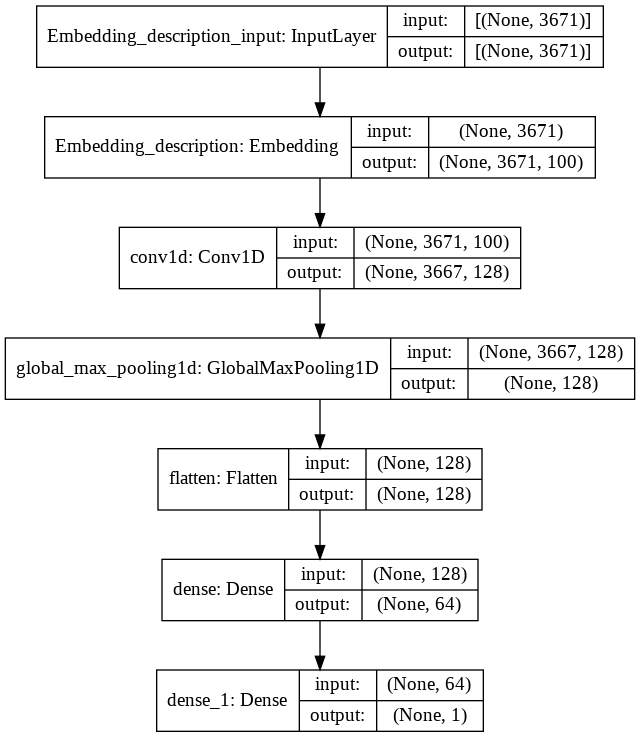
\includegraphics[width=0.60\textwidth]{4/figures/model_cnn_description.png}
		\caption[Arquitectura de modelo CNN para las descripciones]{Arquitectura de modelo CNN para las descripciones.\\
			Fuente: Elaboración propia.}
		\label{4:fig35}
	\end{center}
\end{figure}

Esta red se compone de una capa de incrustación de palabras o \textit{Embedding} alimentada por los datos de entrada en la primera capa \textit{InputLayer} de dimensión de 3,671 vectores de palabras (la mayor longitud de palabras de todas las descripciones), la cual genera como salida una matriz de 3,671 por 100 (número de columnas de incrustaciones de GloVe). Para esta capa se entrenarán 14,827,000 parámetros como resultado del producto de las 100 columnas mencionadas y 148,270 como el tamaño del vocabulario entrenado.

La siguiente capa es la Convolución en 1 dimensión o \textit{Conv1D} (usado frecuentemente para extraer características de datos de textos por ser unidimensionales) que, con 128 características, 5 de tamaño de kernel y función de activación \textit{\textbf{relu}}, generó una salida de 3,667 por 128; así como 64,128 parámetros entrenables.

A continuación, le sigue la capa de reducción \textit{GlobalMaxPooling}. Al igual que en la convolución, esta también fue unidimensional y se caracteriza por realizar agrupamiento global basado en el valor máximo de los bloques seleccionados para reducir el tamaño del vector generado.

Esta nueva salida pasa por la capa de aplanamiento o \textit{Flatten}, en donde se multiplican las filas y columnas y tener un solo vector. Esta sirve para conectar con las 64 neuronas de la nueva capa densa y función de activación \textit{\textbf{tanh}}, agregada con el fin de mejorar la performance del modelo. Según \cite{tec_brownlee2019vanishing_gradients}, se puede considerar el uso tanto de una función \textit{relu} como una función \textit{tanh} cuando se presente la desaparición de grandientes al propagar hacia atrás a mayor cantidad de capas, hecho presentado en los experimentos. Si bien menciona que el uso de la función tangente hiperbólica en capas ocultas resultó una buena práctica durante las décadas de 1990 y 2000, teniendo mejor rendimiento que la función logística, afirma que ambas son dos opciones válidas para problemas de redes neuronales profundas. Por lo tanto, el criterio para considerar una función \textit{tanh} en la investigación obedece a un mejor desempeño en 2\% más de exactitud en el entrenamiento que utilizando la función \textit{relu}.

Finalmente, la arquitectura culmina con la última capa con función de activación \textit{\textbf{sigmoid}} para regular el valor de salida entre 0 y 1, ya que, al tratarse de un problema de clasificación binaria (predecir si un proyecto será financiado: exitoso, de lo contrario: fracasado), cuenta con solo 1 neurona y su parámetro de pérdida es \textit{binary\_crossentropy}. El resumen de todo lo anterior explicado se encuentra en el Anexo \ref{anexo7}.

\textbf{Actividad 3: Desarrollar modelo predictivo de Comentarios}
\\
Al igual que en el modelo de descripciones de proyectos, se creó un diccionario de palabras con la data luego de tokenizar y codificarlas con las mismas funciones y librerías. Sin embargo, a diferencia del anterior modelo, la longitud de la matriz para el rellenado de ceros con el fin de homogenizar el tamaño de cada vector de incrustaciones se limitó a las 5,000 últimas palabras de una oración (parámetro \textbf{padding=`post'} de la función \textit{pad\_sequences}) en lugar de la longitud máxima dado que ésta representa una cantidad considerable (30,072) como para utilizar todos los recursos del entorno de ejecución.

De igual manera, se creó una matriz de incrustaciones de palabras usando GloVe y se diseñó una arquitectura basada en una Red Neuronal Recurrente (RNN por sus siglas en inglés) ilustrada en la Figura \ref{4:fig36}.

\begin{figure}[!ht]
	\begin{center}
		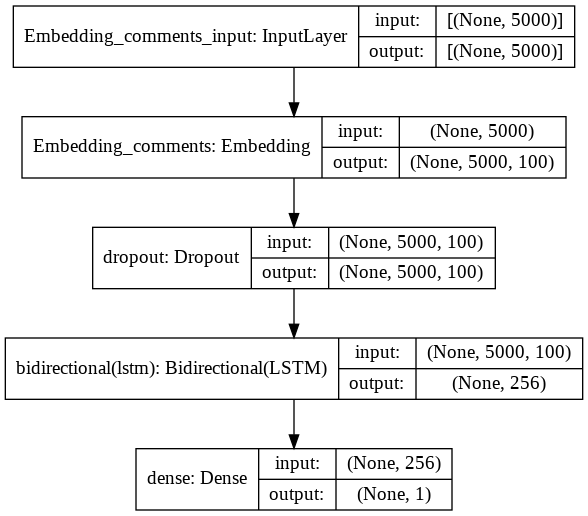
\includegraphics[width=0.60\textwidth]{4/figures/model_rnn_comments.png}
		\caption[Arquitectura de modelo RNN para los comentarios]{Arquitectura de modelo RNN para los comentarios.\\
			Fuente: Elaboración propia.}
		\label{4:fig36}
	\end{center}
\end{figure}

Existe una similitud de estructura en las 2 primeras capas con las del modelo de descripción. Luego de la capa de incrustaciones o \textit{Embedding}, para reducir las conexiones entre neuronas se añadió 1 capa de desactivación o \textit{Dropout}.

A continuación, los vectores de palabras ingresan a la capa de la red neuronal recurrente \textit{LSTM}. Para este caso, se consideró envolverla dentro de una Red Bidireccional de 128 neuronas, ya que como se explicó en el Marco Teórico del Capítulo II sobre las RNN Bidireccionales, este tipo es una mejora de la LSTM tradicional al entrenar 2 juntas (la segunda representa una copia invertida de la secuencia de entrada) en donde cada capa ahora puede considerar también información de las capas siguientes junto con la información de las previas que ya tenía en cuenta, es decir, toma información de 2 direcciones \parencite{tec_brownlee2017bidirectional_lstm}.

Finalmente, el modelo culmina con una capa densa en donde recibe 256 valores de entrada (2*128 de la capa Bidireccional LSTM) y utiliza la función de activación \textit{sigmoid} para transformar el valor final entre 0 y 1. El resumen de lo anterior se encuentra en el Anexo \ref{anexo8}.

Antes de continuar con el desarrollo del modelo de Aprendizaje Profundo Multimodal, en la Tabla \ref{4:table3} se presentan las variables de las modalidades que se usaron para entrenarlo. Estas se seleccionaron de acuerdo al Benchmarking aplicado a los antecedentes en el Capítulo II.

\begin{table}[h!]
	\caption[Diccionario de datos del conjunto final entrenado]{Diccionario de datos del conjunto final entrenado.}
	\label{4:table3}
	\centering
	\small
	\begin{tabular}{ m{3cm}m{9.5cm}m{2.5cm} }
		\specialrule{.1em}{.05em}{.05em}
		\Centering{Variable}& \Centering{Detalle}& \Centering{Tipo de dato}
		\\
		\specialrule{.1em}{.05em}{.05em}
		\multicolumn{3}{c}{Variables independientes} \\
		\hline
		goal &	Monto de la meta de financiamiento del proyecto. &	float64 \\
		%\hline
		completeness & Porcentaje de financiamiento o completitud. & float64 \\
		%\hline
		duration &	Duración de la campaña (en días). &	int64 \\
		%\hline
		pledges\_num &	Cantidad de montos disponibles para contribuir. &	int64 \\
		%\hline
		pledged &	Monto contribuído en la campaña. &	float64 \\
		%\hline
		pledges\_median &	Mediana de montos disponibles para contribuir. &	float64 \\
		%\hline
		description &	Descripción del proyecto. &	object \\
		%\hline
		comments & Comentarios de patrocinadores sobre el proyecto. & object \\
		\hline
		\multicolumn{3}{c}{Variable dependiente} \\
		\hline
		state & Estado de financiamiento del proyecto. & object \\
		\specialrule{.1em}{.05em}{.05em}
	\end{tabular}
	%\par	%%Salto de linea
	%\bigskip
	\begin{flushleft}	%%Alinear a la izquierda sin justificar
		\small Fuente: Elaboración propia.
	\end{flushleft}
\end{table}

Los autores citados por cada variable utilizada se mencionan a continuación:
\begin{itemize}
	\item \textbf{goal}: \cite{pr_chen2013kickpredict}, \cite{pr_mitra2014phrases}, \cite{pr_zhou2015projectdesc}, \cite{pr_chen2015predcrowd}, \cite{pr_li2016predcrowd}, \cite{pr_yuan2016textanalytics}, \cite{pr_sawhney2016usingLT}, \cite{pr_kaur2017socmedcrowd}, \cite{pr_kamath2018suplearn}, \cite{pr_yu2018deeplearning}, \cite{pr_jin2019dayssuccess}, \cite{pr_cheng2019deeplearning}.
	\item \textbf{completeness}: \cite{pr_chen2015predcrowd}.
	\item \textbf{duration}: \cite{pr_mitra2014phrases}, \cite{pr_zhou2015projectdesc}, \cite{pr_li2016predcrowd}, \cite{pr_sawhney2016usingLT}, \cite{pr_kaur2017socmedcrowd}, \cite{pr_kamath2018suplearn}, \cite{pr_yu2018deeplearning}, \cite{pr_jin2019dayssuccess}.
	\item \textbf{pledges\_num}: \cite{pr_chen2013kickpredict}, \cite{pr_mitra2014phrases}, \cite{pr_chen2015predcrowd}, \cite{pr_yuan2016textanalytics}, \cite{pr_jin2019dayssuccess}.
	\item \textbf{pledged}: \cite{pr_chen2013kickpredict}, \cite{pr_li2016predcrowd}, \cite{pr_kamath2018suplearn}.
	\item \textbf{pledges\_median}: \cite{pr_chen2015predcrowd}*, \cite{pr_jin2019dayssuccess}*.
	\item \textbf{description}: \cite{pr_mitra2014phrases}, \cite{pr_zhou2015projectdesc}, \cite{pr_yuan2016textanalytics}, \cite{pr_sawhney2016usingLT}, \cite{pr_kamath2018suplearn}, \cite{pr_lee2018contentDL}, \cite{pr_jin2019dayssuccess}, \cite{pr_cheng2019deeplearning}, \cite{pr_chen2019keywords_crowdfunding}, \cite{pr_chaichi2019nlp_3dprinting}.
	\item \textbf{comments}: \cite{pr_li2016predcrowd}, \cite{pr_kaur2017socmedcrowd}, \cite{pr_lee2018contentDL}, \cite{pr_jin2019dayssuccess}.
\end{itemize}

Si bien en los respectivos antecedentes marcados en (*) figuran el promedio de los montos disponibles para patrocinar, se usó la mediana en vez de la media ya que presentó mejor performance en los experimentos.

\begin{landscape}
	\textbf{Actividad 4: Desarrollar modelo ensamblado apilado}
	\\
	Una vez construidos los modelos para cada modalidad (metainformación, descripción y comentarios), se construyó un modelo de Aprendizaje Profundo Multimodal ilustrado en la Figura \ref{4:fig37}.
	
	\begin{figure}[!ht]
		\begin{center}
			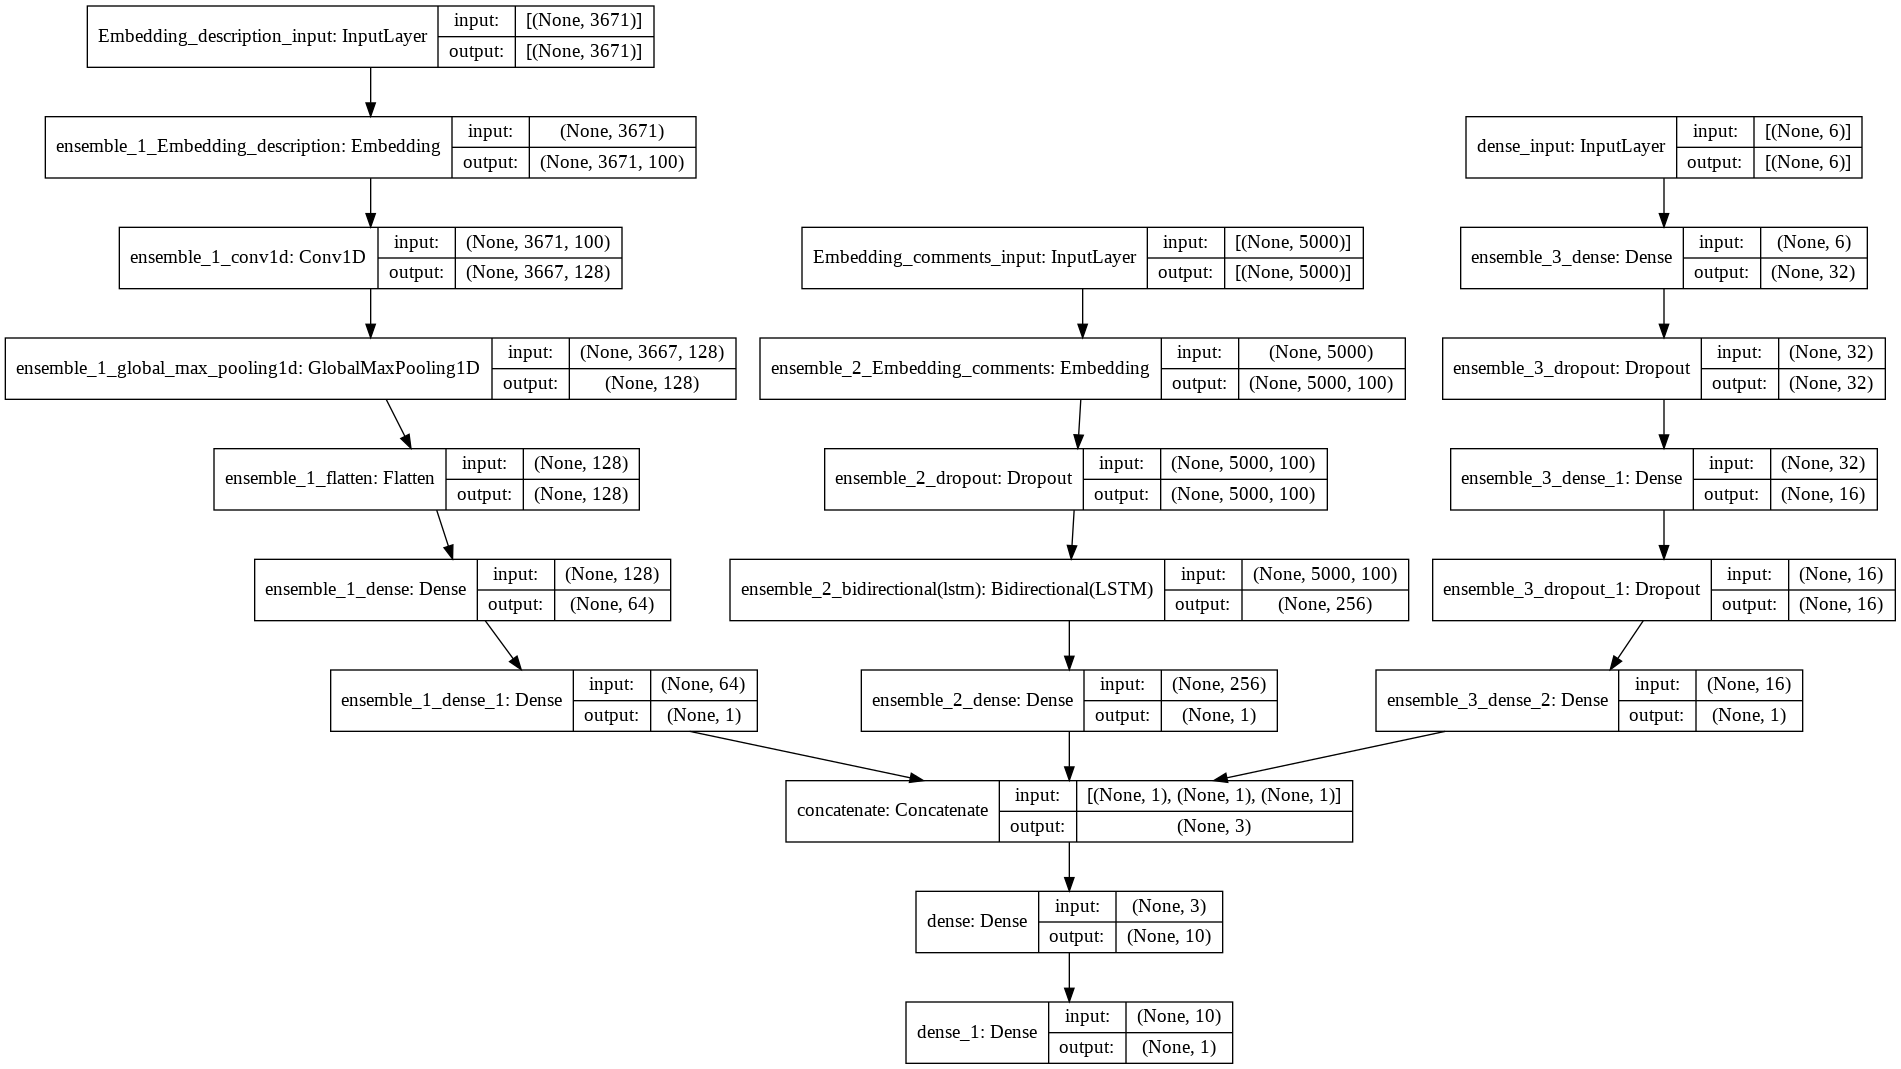
\includegraphics[width=1.20\textwidth]{4/figures/final_stacked_model.png}
			\caption[Arquitectura del modelo apilado final The Hydra]{Arquitectura del modelo apilado final The Hydra.\\
				Fuente: Elaboración propia.}
			\label{4:fig37}
		\end{center}
	\end{figure}
	
\end{landscape}

La finalidad de este modelo apilado de múltiples cabezas es aprender la mejor manera de combinar las predicciones de cada submodelo para lograr un mayor rendimiento y clasificar mejor la variable dependiente que cada modalidad.

A este modelo se le denominó “\textit{The Hydra}” (La Hidra por su traducción al español) en referencia al monstruo mitológico del lago de Lerna, con 7 cabezas que renacían a medida que se cortaban \parencite{ot_rae_hidra}.

Al tratarse de un modelo ensamblado apilado, las salidas de cada modelo se concatenaron en una capa debajo de estos, generando 3 valores de entrada para una penúltima capa densa con 10 neuronas de salida y una función de activación \textit{\textbf{relu}}. El modelo apilado culmina con una capa densa de 1 salida y asignándose la función Sigmoide para generar probabilidades entre 0 y 1, los valores de Fracasado o Exitoso respectivamente.

Previo a la compilación del modelo final, se repitió el ejercicio de cada modelo cargado asignar los parámetro de pérdida \textit{binary\_crossentropy} para la clasificación binaria, \textit{accuracy} (exactitud) para la métrica del entrenamiento, pesos balanceados para las clases de la variable \textit{state} (0.6987077585764833 para 0 y 1.7581290322580645 para 1), y optimizador \textit{Adam} con la variante de asignarle el ratio de aprendizaje y también de decaimiento de 0.00005. El resumen de todo los parámetros anteriores se encuentra en el Anexo \ref{anexo9}.


\section{Evaluación}
Como parte de la aplicación de la metodología CRISP-DM, explicada en el sexto subcapítulo del Capítulo III, se mencionaron las métricas usadas en la literatura. La más recurrente fue la exactitud. Dado que la librería Scikit-learn cuenta con un reporte de clasificación con esta métrica y otras 4 más como la precisión, sensibilidad, puntaje F1 y AUC, además que la distribución de proyectos por su estado de financiamiento es desbalanceada y se necesita más de un indicador para poder evaluar y comparar, se decidió usar estas 5 teniendo como referencias a los autores \citeauthor{pr_beckwith2016predcrowd} (quinto antecedente), \citeauthor{pr_yuan2016textanalytics}* (séptimo antecedente), \citeauthor{pr_kaur2017socmedcrowd} (noveno antecedente), \citeauthor{pr_cheng2019deeplearning} (decimocuarto antecedente), y \citeauthor{pr_chen2019keywords_crowdfunding}** (decimoquinto antecedente).

En el antecedente marcado en (*), los modelos no fueron evaluados por AUC; mientras que en (**), las métricas precisión y AUC no fueron tomadas en cuenta.

\textbf{Actividad 1: Evaluar desempeño del modelo predictivo de Metainformación}
\\
Luego de 19 épocas, con un promedio de 3 segundos de entrenamiento cada una, el modelo dejó de entrenar dado que durante 7 épocas no registró una reducción en el valor de la pérdida del subconjunto de validación, a pesar de que hace 3 épocas se redujo su tasa de aprendizaje.

Así, de acuerdo a la Figura \ref{5:fig1}, en la época 11 se registran los mejores valores de exactitud y pérdida para el subconjunto de validación, alcanzando 0.9523 y 0.1246 respectivamente.

\begin{figure}[!ht]
	\begin{center}
		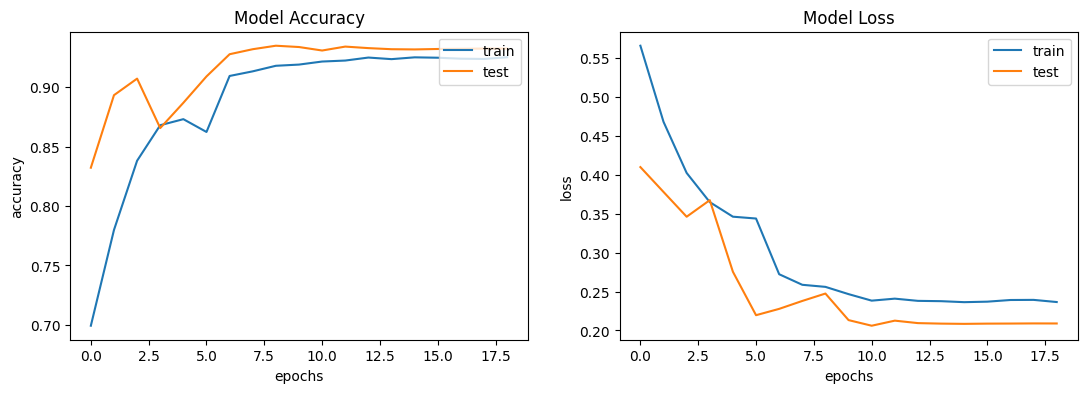
\includegraphics[width=1\textwidth]{5/figures/metadata_model_acc_loss.png}
		\caption[Exactitud y pérdida respectivamente de los subconjuntos de entrenamiento y validación para el modelo MLP de metadata con 100 épocas]{Exactitud y pérdida respectivamente de los subconjuntos de entrenamiento y validación para el modelo MLP de metadata con 100 épocas.\\
		Fuente: Elaboración propia.}
		\label{5:fig1}
	\end{center}
\end{figure}

La matriz de confusión resultante se representa en la Figura \ref{5:fig2}.

\begin{figure}[!ht]
	\begin{center}
		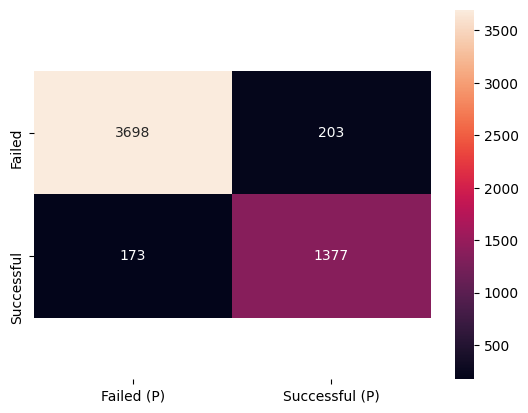
\includegraphics[width=0.75\textwidth]{5/figures/metadata_confusion_matrix.png}
		\caption[Matriz de confusión para el modelo de metadata]{Matriz de confusión para el modelo de metadata.\\
		Fuente: Elaboración propia.}
		\label{5:fig2}
	\end{center}
\end{figure}

De esta matriz, se derivan los resultados de la Tabla \ref{5:table1} y el AUC en la Figura \ref{5:fig3}.

\begin{table}[h!]
	\caption[Informe de clasificación para el modelo de metadata]{Informe de clasificación para el modelo de metadata.}
	\label{5:table1}
	\centering
	\small
	\begin{tabular}{ m{4.5cm}M{2.5cm}M{2.5cm}M{2.5cm}M{2.5cm} }
		\specialrule{.1em}{.05em}{.05em}
		\Centering{Valor}& \Centering{Precisión}& \Centering{Sensibilidad}& \Centering{Puntaje F1}& \Centering {Muestras}\\
		\specialrule{.1em}{.05em}{.05em}
		Fracasado & 0.96 & 0.95 & 0.95 & 3,901 \\
		%\hline
		Exitoso & 0.87 & 0.89 & 0.88 & 1,550 \\
		\hline
		%\multicolumn{5}{c}{ } \\
		%\hline
		Exactitud &  &	 & 0.93 & 5,451 \\
		\hline
		Promedio macro & 0.91 & 0.92 & 0.92 & 5,451 \\
		%\hline
		Promedio ponderado & 0.93 & 0.93 & 0.93 & 5,451 \\
		\specialrule{.1em}{.05em}{.05em}
	\end{tabular}
	%\par	%%Salto de linea
	%\bigskip
	\begin{flushleft}	%%Alinear a la izquierda sin justificar
		\small Fuente: Elaboración propia.
	\end{flushleft}
\end{table}

\begin{itemize}
	\item El ratio de exactitud se interpreta como: El 93\% de los proyectos de la muestra fueron predichos correctamente.
	\item El ratio de precisión para los positivos (\textit{Successful}) se interpreta como: El 87\% de los proyectos exitosos predichos de la muestra fueron clasificados correctamente. 
	\item El ratio de sensibilidad para los positivos (\textit{Successful}) se interpreta como: El 89\% de los proyectos exitosos reales de la muestra fueron clasificados correctamente.
	\item El ratio de Puntaje F1 para los positivos (\textit{Successful}) representa un balance entre las 2 métricas anteriores. En la tabla se observa que su valor es de 88\%, lo cual indica que en general, el modelo mantiene un alto rendimiento.
\end{itemize}

\begin{figure}[!ht]
	\begin{center}
		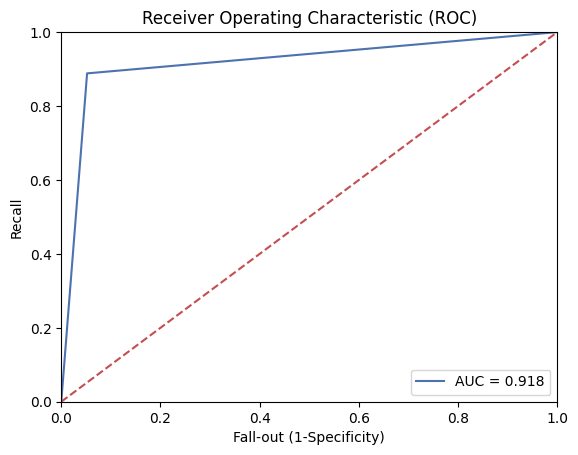
\includegraphics[width=0.56\textwidth]{5/figures/metadata_auc.png}
		\caption[Área bajo la curva ROC de modelo de metadata]{Área bajo la curva ROC de modelo de metadata.\\
		Fuente: Elaboración propia.}
		\label{5:fig3}
	\end{center}
\end{figure}

El área bajo la Curva ROC presenta un valor de aproximadamente 92\%, del cual se observa en el gráfico que su sensibilidad es muy alta y el ratio de Falsa Alarma es casi nulo. De acuerdo con \cite{bk_britos2006datamining}, el poder discriminante del modelo es excelente.

\textbf{Actividad 2: Evaluar desempeño del modelo predictivo de Descripción}
\\
Luego de 82 épocas, con un promedio de 106 segundos de entrenamiento cada una, el modelo dejó de entrenar dado que durante 10 épocas no registró una reducción en el valor de la pérdida del subconjunto de validación, a pesar de que hace 5 épocas se redujo su tasa de aprendizaje.

Así, de acuerdo a la Figura \ref{5:fig4}, en la época 72 se registran los mejores valores de exactitud y pérdida para el subconjunto de validación, alcanzando 0.7683 y 0.4901 respectivamente.

\begin{figure}[!ht]
	\begin{center}
		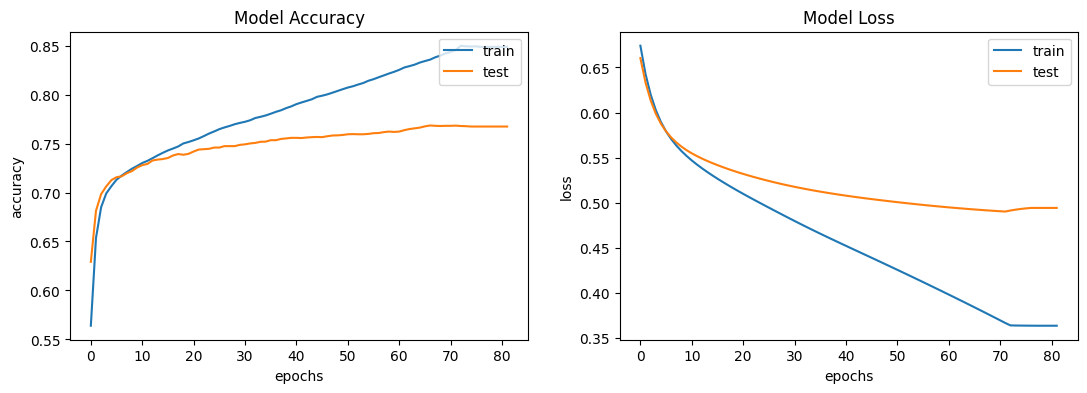
\includegraphics[width=1\textwidth]{5/figures/description_model_acc_loss.png}
		\caption[Exactitud y pérdida respectivamente de los subconjuntos de entrenamiento y validación para el modelo CNN de descripciones con 100 épocas]{Exactitud y pérdida respectivamente de los subconjuntos de entrenamiento y validación para el modelo CNN de descripciones con 100 épocas.\\
		Fuente: Elaboración propia.}
		\label{5:fig4}
	\end{center}
\end{figure}

La matriz de confusión resultante se representa en la Figura \ref{5:fig5}.

\begin{figure}[!ht]
	\begin{center}
		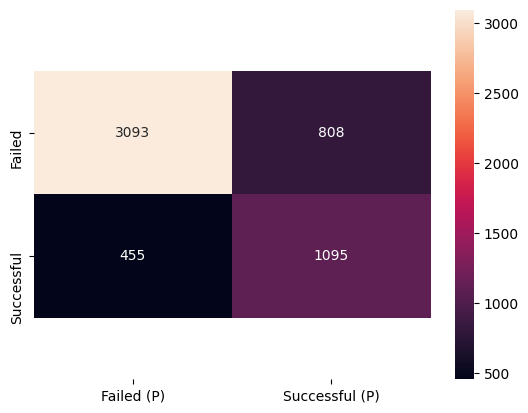
\includegraphics[width=0.75\textwidth]{5/figures/description_confusion_matrix.png}
		\caption[Matriz de confusión para el modelo de descripciones]{Matriz de confusión para el modelo de descripciones.\\
		Fuente: Elaboración propia.}
		\label{5:fig5}
	\end{center}
\end{figure}

De esta matriz, se derivan los resultados de la Tabla \ref{5:table2} y el AUC en la Figura \ref{5:fig6}.

\begin{table}[h!]
	\caption[Informe de clasificación para el modelo de descripciones]{Informe de clasificación para el modelo de descripciones.}
	\label{5:table2}
	\centering
	\small
	\begin{tabular}{ m{4.5cm}M{2.5cm}M{2.5cm}M{2.5cm}M{2.5cm} }
		\specialrule{.1em}{.05em}{.05em}
		\Centering{Valor}& \Centering{Precisión}& \Centering{Sensibilidad}& \Centering{Puntaje F1}& \Centering{Muestras}\\
		\specialrule{.1em}{.05em}{.05em}
		Fracasado & 0.87 & 0.79 & 0.83 & 3,901 \\
		%\hline
		Exitoso & 0.58 & 0.71 & 0.63 & 1,550 \\
		\hline
		%\multicolumn{5}{c}{ } \\
		%\hline
		Exactitud &  &	 & 0.77 & 5,451 \\
		\hline
		Promedio macro & 0.72 & 0.75 & 0.73 & 5,451 \\
		%\hline
		Promedio ponderado & 0.79 & 0.77 & 0.77 & 5,451 \\
		\specialrule{.1em}{.05em}{.05em}
	\end{tabular}
	%\par	%%Salto de linea
	%\bigskip
	\begin{flushleft}	%%Alinear a la izquierda sin justificar
		\small Fuente: Elaboración propia.
	\end{flushleft}
\end{table}

\begin{itemize}
	\item El ratio de exactitud se interpreta como: El 77\% de los proyectos de la muestra fueron predichos correctamente.
	\item El ratio de precisión para los positivos (\textit{Successful}) se interpreta como: El 58\% de los proyectos exitosos predichos de la muestra fueron clasificados correctamente. 
	\item El ratio de sensibilidad para los positivos (\textit{Successful}) se interpreta como: El 71\% de los proyectos exitosos reales de la muestra fueron clasificados correctamente.
	\item El ratio de Puntaje F1 para los positivos (\textit{Successful}) representa un balance entre las 2 métricas anteriores. En la tabla se observa que su valor es de 63\%, lo cual indica que en general, el modelo presenta un rendimiento regular.
\end{itemize}

\begin{figure}[!ht]
	\begin{center}
		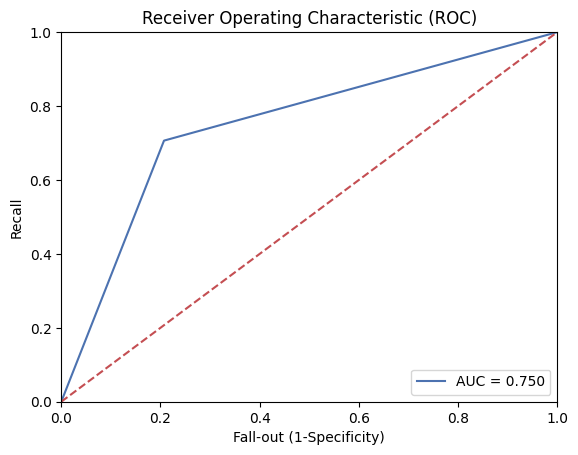
\includegraphics[width=0.56\textwidth]{5/figures/description_auc.png}
		\caption[Área bajo la curva ROC de modelo de descripciones]{Área bajo la curva ROC de modelo de descripciones.\\
		Fuente: Elaboración propia.}
		\label{5:fig6}
	\end{center}
\end{figure}

El área bajo la Curva ROC presenta un valor de aproximadamente 75\%, del cual se observa en el gráfico que su sensibilidad es medianamente alta y el ratio de Falsa Alarma es medianamente baja. De acuerdo con \cite{bk_britos2006datamining}, el poder discriminante del modelo es aceptable .

\newpage
\textbf{Actividad 3: Evaluar desempeño del modelo predictivo de Comentarios}
\\
Luego de 43 épocas, con 77 segundos en promedio de entrenamiento cada una, el modelo dejó de entrenar dado que durante 10 épocas no registró una reducción en el valor de la pérdida del subconjunto de validación, por más que 1 época antes se había reducido su tasa de aprendizaje.

Así, de acuerdo a la Figura \ref{5:fig7}, en la época 33 se registran los mejores valores de exactitud y pérdida para el subconjunto de validación, alcanzando 0.8510 y 0.4472 respectivamente.

\begin{figure}[!ht]
	\begin{center}
		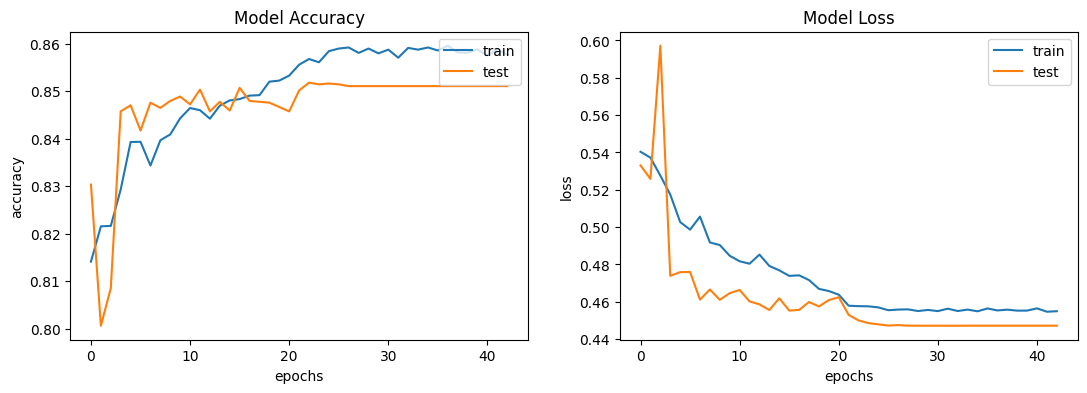
\includegraphics[width=1\textwidth]{5/figures/comments_model_acc_loss.png}
		\caption[Exactitud y pérdida respectivamente de los subconjuntos de entrenamiento y validación para el modelo RNN de comentarios con 50 épocas]{Exactitud y pérdida respectivamente de los subconjuntos de entrenamiento y validación para el modelo RNN de comentarios con 50 épocas.\\
		Fuente: Elaboración propia.}
		\label{5:fig7}
	\end{center}
\end{figure}

La matriz de confusión resultante se representa en la Figura \ref{5:fig8}.
\begin{figure}[!ht]
	\begin{center}
		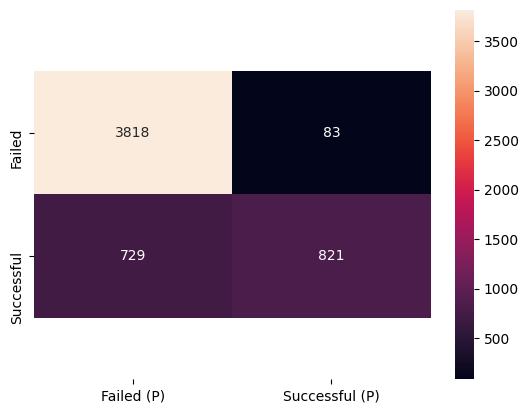
\includegraphics[width=0.75\textwidth]{5/figures/comments_confusion_matrix.png}
		\caption[Matriz de confusión para el modelo de comentarios]{Matriz de confusión para el modelo de comentarios.\\
		Fuente: Elaboración propia.}
		\label{5:fig8}
	\end{center}
\end{figure}

De esta matriz, se derivan los resultados de la Tabla \ref{5:table3} y el AUC en la Figura \ref{5:fig9}.

\begin{table}[h!]
	\caption[Informe de clasificación para el modelo de comentarios]{Informe de clasificación para el modelo de comentarios.}
	\label{5:table3}
	\centering
	\small
	\begin{tabular}{ m{4.5cm}M{2.5cm}M{2.5cm}M{2.5cm}M{2.5cm} }
		\specialrule{.1em}{.05em}{.05em}
		\Centering{Valor}& \Centering{Precisión}& \Centering{Sensibilidad}& \Centering{Puntaje F1}& \Centering{Muestras}\\
		\specialrule{.1em}{.05em}{.05em}
		Fracasado & 0.84 & 0.98 & 0.90 & 3,901 \\
		%\hline
		Exitoso & 0.91 & 0.53 & 0.67 & 1,550 \\
		\hline
		%\multicolumn{5}{c}{ } \\
		%\hline
		Exactitud &  &	 & 0.85 & 5,451 \\
		\hline
		Promedio macro & 0.87 & 0.75 & 0.79 & 5,451 \\
		%\hline
		Promedio ponderado & 0.86 & 0.85 & 0.84 & 5,451 \\
		\specialrule{.1em}{.05em}{.05em}
	\end{tabular}
	%\par	%%Salto de linea
	%\bigskip
	\begin{flushleft}	%%Alinear a la izquierda sin justificar
		\small Fuente: Elaboración propia.
	\end{flushleft}
\end{table}

\begin{itemize}
	\item El ratio de exactitud se interpreta como: El 85\% de los proyectos de la muestra fueron predichos correctamente.
	\item El ratio de precisión para los positivos (\textit{Successful}) se interpreta como: El 91\% de los proyectos exitosos predichos de la muestra fueron clasificados correctamente. 
	\item El ratio de sensibilidad para los positivos (\textit{Successful}) se interpreta como: El 53\% de los proyectos exitosos reales de la muestra fueron clasificados correctamente.
	\item El ratio de Puntaje F1 para los positivos (\textit{Successful}) representa un balance entre las 2 métricas anteriores. En la tabla se observa que su valor es de 67\%, lo cual indica que en general, el modelo presenta un rendimiento regular.
\end{itemize}

\begin{figure}[!ht]
	\begin{center}
		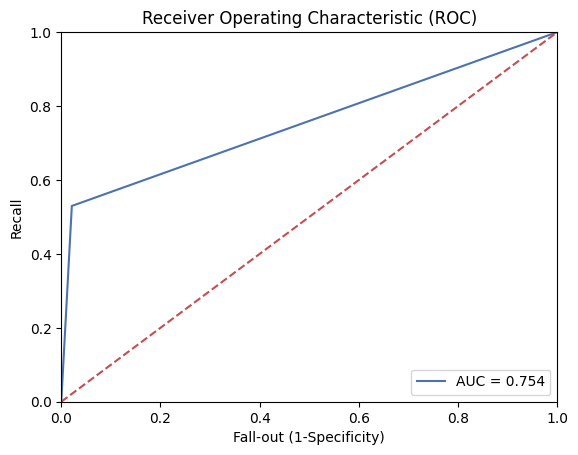
\includegraphics[width=0.57\textwidth]{5/figures/comments_auc.png}
		\caption[Área bajo la curva de modelo de comentarios]{Área bajo la curva de modelo de comentarios.\\
		Fuente: Elaboración propia.}
		\label{5:fig9}
	\end{center}
\end{figure}

El área bajo la Curva ROC presenta un valor de aproximadamente 75\%, del cual se observa en el gráfico que su sensibilidad es baja pero su ratio de Falsa Alarma es casi nulo. De acuerdo con \cite{bk_britos2006datamining}, el poder discriminante del modelo es aceptable.

%\newpage
\textbf{Actividad 4: Evaluar desempeño del modelo ensamblado apilado}
\\
Luego de 13 épocas, con 152 segundos de entrenamientos cada una, el modelo dejó de entrenar dado que durante 10 épocas no registró una reducción en el valor de la pérdida del subconjunto de validación, a pesar de que hace 2 épocas se redujo su tasa de aprendizaje.

Así, de acuerdo a la Figura \ref{5:fig10}, en la época 3 se registran los mejores valores de exactitud y pérdida para el subconjunto de validación, alcanzando 0.9336 y 0.1810 respectivamente.

\begin{figure}[!ht]
	\begin{center}
		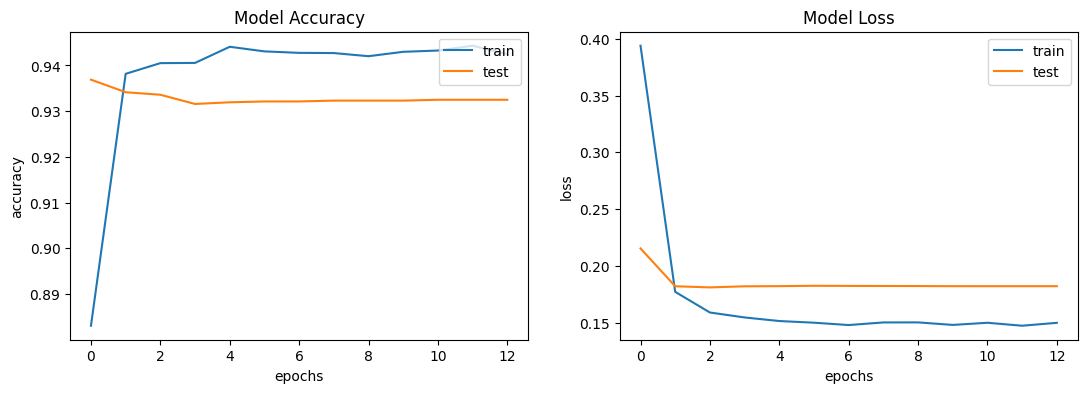
\includegraphics[width=1\textwidth]{5/figures/stacked_model_acc_loss.png}
		\caption[Exactitud y pérdida respectivamente de los subconjuntos de entrenamiento y validación para el modelo apilado con 200 épocas]{Exactitud y pérdida respectivamente de los subconjuntos de entrenamiento y validación para el modelo apilado con 200 épocas.\\
		Fuente: Elaboración propia.}
		\label{5:fig10}
	\end{center}
\end{figure}

\newpage
La matriz de confusión resultante se representa en la Figura \ref{5:fig11}.
\begin{figure}[!ht]
	\begin{center}
		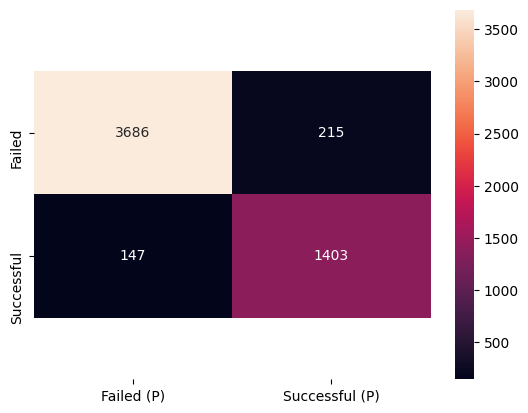
\includegraphics[width=0.75\textwidth]{5/figures/stacked_confusion_matrix.png}
		\caption[Matriz de confusión para el modelo apilado]{Matriz de confusión para el modelo apilado.\\
		Fuente: Elaboración propia.}
		\label{5:fig11}
	\end{center}
\end{figure}

De esta matriz, se derivan los resultados de la Tabla \ref{5:table4} y el AUC en la Figura \ref{5:fig12}.

\begin{table}[h!]
	\caption[Informe de clasificación para el modelo apilado]{Informe de clasificación para el modelo apilado.}
	\label{5:table4}
	\centering
	\small
	\begin{tabular}{ m{4.5cm}M{2.5cm}M{2.5cm}M{2.5cm}M{2.5cm} }
		\specialrule{.1em}{.05em}{.05em}
		\Centering{Valor}& \Centering{Precisión}& \Centering{Sensibilidad}& \Centering{Puntaje F1}& \Centering{Muestras}\\
		\specialrule{.1em}{.05em}{.05em}
		Fracasado & 0.96 & 0.94 & 0.95 & 3,901 \\
		%\hline
		Exitoso & 0.87 & 0.91 & 0.89 & 1,550 \\
		\hline
		%\multicolumn{5}{c}{ } \\
		%\hline
		Exactitud &  &	 & 0.93 & 5,451 \\
		\hline
		Promedio macro & 0.91 & 0.93 & 0.92 & 5,451 \\
		%\hline
		Promedio ponderado & 0.93 & 0.93 & 0.93 & 5,451 \\
		\specialrule{.1em}{.05em}{.05em}
	\end{tabular}
	\par	%%Salto de linea
	\bigskip
	\begin{flushleft}	%%Alinear a la izquierda sin justificar
		\small Fuente: Elaboración propia.
	\end{flushleft}
\end{table}

\begin{itemize}
	\item El ratio de exactitud se interpreta como: El 93\% de los proyectos de la muestra fueron predichos correctamente.
	\item El ratio de precisión para los positivos (\textit{Successful}) se interpreta como: El 87\% de los proyectos exitosos predichos de la muestra fueron clasificados correctamente. 
	\item El ratio de sensibilidad para los positivos (\textit{Successful}) se interpreta como: El 91\% de los proyectos exitosos reales de la muestra fueron clasificados correctamente.
	\item El ratio de Puntaje F1 para los positivos (\textit{Successful}) representa un balance entre las 2 métricas anteriores. En la tabla se observa que su valor es de 89\%, lo cual indica que en general, el modelo presenta un rendimiento regular.
\end{itemize}

\begin{figure}[!ht]
	\begin{center}
		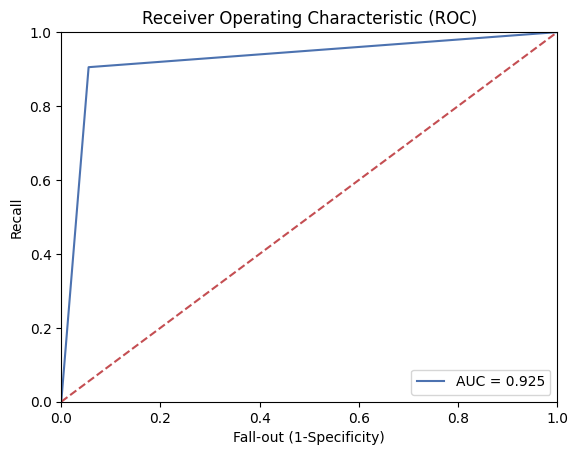
\includegraphics[width=0.57\textwidth]{5/figures/stacked_auc.png}
		\caption[Área bajo la curva de modelo apilado]{Área bajo la curva de modelo apilado.\\
		Fuente: Elaboración propia.}
		\label{5:fig12}
	\end{center}
\end{figure}

El área bajo la Curva ROC presenta un valor aproximado de 93\%, del cual se observa en el gráfico que su sensibilidad es muy alta y su ratio de Falsa Alarma es casi nulo. De acuerdo con \cite{bk_britos2006datamining}, el poder discriminante del modelo es excepcionalmente bueno.

Finalmente, considerando los modelos independientes para cada modalidad, así como un trabajo previo del autor de la presente investigación cuyo trabajo sirvió de base \parencite{pr_puente2019kickstarter_prediction}, se armó el cuadro comparativo de la Tabla \ref{5:table5}.

\begin{table}[h!]
	\caption[Comparación de resultados de modelos propuestos con antecedentes]{Comparación de resultados de modelos propuestos con antecedentes.}
	\label{5:table5}
	\centering
	\small
	\begin{tabular}{llccccc}
		\specialrule{.1em}{.05em}{.05em}
		\multicolumn{2}{c}{Modelos} & Exactitud & Precisión & Sensibilidad & Puntaje F1 & AUC
		\\
		\specialrule{.1em}{.05em}{.05em}
		\multirow{2}{*}{Tesis de pregrado} & Metainformación                                                            & 0.89                                                              & 0.86                                                              & 0.72                                                                 & 0.75                                                               & 0.84                                                        \\
		%\hline
		{} & Descripción                                                         & 0.75                                                              & 0.59                                                              & 0.53                                                                 & 0.35                                                               & 0.68                                                        \\
		\hline
		\multirow{4}{*}{Propuesta} & Metainformación                                                                 & 0.93                                                              & 0.91                                                              & 0.92                                                                 & 0.92                                                               & 0.92                                                        \\
		%\hline
		{} & Descripción                                                               & 0.77                                                              & 0.72                                                              & 0.75                                                                 & 0.73                                                               & 0.75                                                        \\
		%\hline
		{} & Comentarios                                                               & 0.85                                                              & 0.87                                                              & 0.75                                                                 & 0.79                                                               & 0.75                                                        \\
		%\specialrule{.1em}{.05em}{.05em}
		{} & The Hydra & 0.93 & 0.91 & 0.93 & 0.92 & 0.93 \\
		\specialrule{.1em}{.05em}{.05em}
	\end{tabular}
	\par	%%Salto de linea
	\bigskip
	\begin{flushleft}	%%Alinear a la izquierda sin justificar
		\small Fuente: Elaboración propia.
	\end{flushleft}
\end{table}

Los modelos citados de la Tesis de pregrado para Metainformación y Descripción utilizaron una Máquina de Vectores de Soporte (SVM) y una SVM entrenada con el algoritmo TF-IDF, respectivamente.

Para comparar ambas investigaciones, se usaron las mismas bases de datos para las 2 modalidades, con proyectos tecnológicos de Kickstarter finalizados entre 2009 y 2019, así como también las mismas métricas para evaluar cada modelo. El tiempo de entrenamiento en el antecedente mencionado fue mayor (aproximadamente 16 segundos para la metainformación y 4 horas para la descripción), en contraste con los elaborados en este trabajo (aproximadamente 38 segundos para la metainformación y 2 horas y media para la descripción).

Como se observa en la Tabla \ref{5:table5}, a nivel general, la performance de The Hydra fue mejor tanto contra los modelos individuales de cada modalidad (superando en más de 0.03 y más de 0.05 al modelo de comentarios y descripción respectivamente en las 5 métricas, y en 0.01 al de metainformación en AUC) como contra los modelos referenciados en los antecedentes (más de 0.05 en todas las métricas para el modelo de metainformación y más de 0.18 en todas las métricas para el modelo de descripción). El concepto (con otros modelos y variantes en el desarrollo) utilizado en la Tesis de pregrado se basó en el trabajo de los autores \cite{pr_cheng2019deeplearning}, el cual utilizó un marco de trabajo de Aprendizaje Profundo Multimodal (\textit{Multimodal Deep Learning} en inglés), donde se combinan las características de metainformación, descripción e imagen principal del proyecto en la capa totalmente conectada. Sin embargo, en dicha ocasión no se alcanzó lograr los objetivos dado que el modelo de contenido visual presentó problemas para clasificar adecuadamente un proyecto según su estado. Esto se dio en parte a la variedad de imágenes dentro de la misma categoría Tecnología, que contiene asimismo 16 subcategorías, lo cual dificultó en su momento a la red a encontrar patrones a partir de su características. Se decidió, entonces, cambiar el criterio de reemplazar el contenido visual por otra modalidad respaldada por varios antecedentes (enunciados en la descripción del prototipo de investigación del Capítulo III) y que no fue tomada en cuenta en su momento, los comentarios realizados durante la campaña por los patrocinadores del proyecto.

\section{Despliegue}
\textbf{Actividad 1: Diseñar prototipo de sistema con modelo propuesto}
\\
La última fase de la metodología CRISP-DM comienza con el diseño del prototipo que contemplará el sistema conformado por la captura de datos y la predicción del estado de financiamiento de un proyecto consultado. Para ello, previamente se deberán cargarse todos los complementos necesarios para que el modelo de Aprendizaje Profundo Multimodal funcione correctamente. Desde librerías de Python que incluyen elementos utilizados en la recolección de datos como Selenium y las librerías de Keras para la carga de las capas del modelo, hasta algoritmos usados para la limpieza de texto como NLTK y las métricas de clasificación por parte de Scikit-learn.

Luego de la anterior acción, se diseñó el código para ejecutar el proceso de la Figura \ref{3:fig10} explicado en el Capítulo III. El código del prototipo y sus respectivos elementos pueden ser descargados desde link \textbf{\url{https://www.kaggle.com/alonsopuente/tesis-titulacion-demo}}

\textbf{Actividad 2: Ejecutar prototipo con proyectos tecnológicos vigentes}
\\
Una vez diseñado el proceso del prototipo, el software es ejecutado localmente desde Jupyter Notebook y recibe como dato de entrada el enlace web de un proyecto vigente en Kickstarter, representado en la Figura \ref{4:fig38}.

\begin{figure}[!ht]
	\begin{center}
		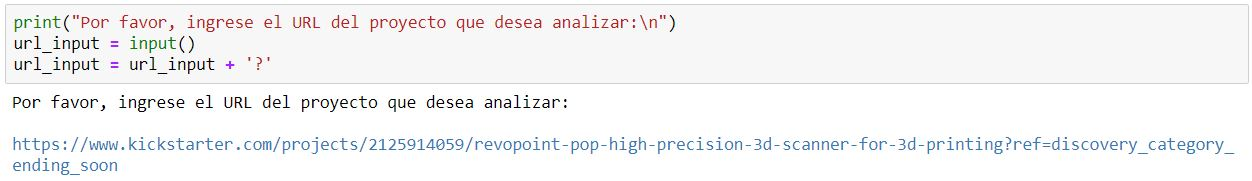
\includegraphics[width=1.10\textwidth]{4/figures/prototipo_input_project1.jpg}
		\caption[Proyecto consultado para la demostración. Captura de pantalla: 15/02/21]{Proyecto consultado para la demostración. Captura de pantalla: 15/02/21.\\
			Fuente: Elaboración propia.}
		\label{4:fig38}
	\end{center}
\end{figure}

Uno de los experimentos hechos el 23 de enero del 2021 se realizó con la campaña vigente de ejemplo de la Figura \ref{4:fig39}.

\begin{figure}[!ht]
	\begin{center}
		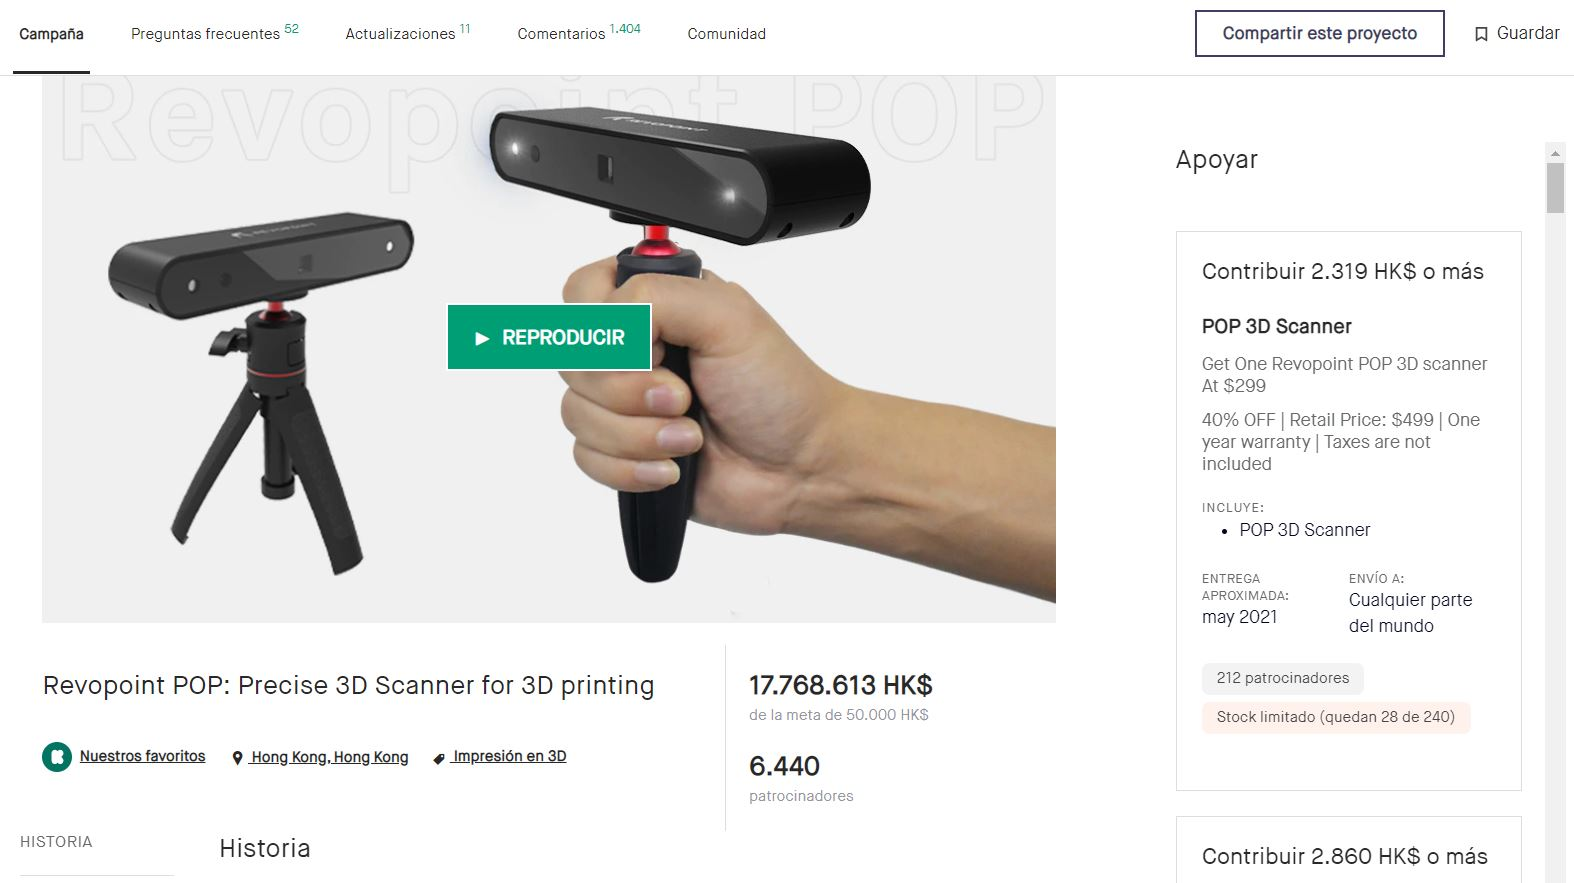
\includegraphics[width=1\textwidth]{4/figures/example_project_150221.jpg}
		\caption[Campaña del proyecto consultado. Captura de pantalla: 15/02/21]{Campaña del proyecto consultado. Captura de pantalla: 15/02/21.\\
			Fuente: Elaboración propia.}
		\label{4:fig39}
	\end{center}
\end{figure}

La primera acción hecha por el sistema fue extraer la metainformación, descripción y comentarios del proyecto desde el ingreso al URL por un navegador. Debido al cambio de políticas de acceso a la plataforma en 2020, Kickstarter detecta la presencia de bots y restringe la navegación usando CAPTCHAs para evitar su accionar. Algunas veces fue detectado el bot del sistema. Ante ello, la única acción manual por parte del usuario en el sistema se da en este paso presionando por 5 segundos el botón de “\textit{I'm a human}” (Soy humano por su traducción al español) que se muestra en la ventana. Desde este punto, luego de ingresar al enlace de la campaña del proyecto, el sistema primero se redirige a la sección de la metainformación y extrae las variables usadas para el entrenamiento del modelo. Del mismo modo, repite esta secuencia para la descripción y los comentarios.

Los datos extraídos de cada modalidad se muestran en la Figura \ref{4:fig40} respectivamente.

\begin{figure}[!ht]
	\centering
	\small
	\begin{subfigure}{1.0\textwidth}
		\centering
		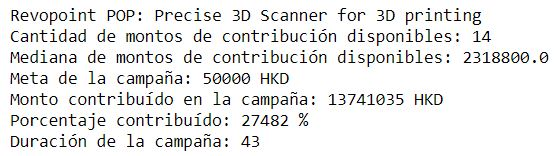
\includegraphics[width=0.75\linewidth]{4/figures/metadata_scraped_project.jpg}
		\caption{Metainformación}
	\end{subfigure}
	\begin{subfigure}{.50\textwidth}
		\centering
		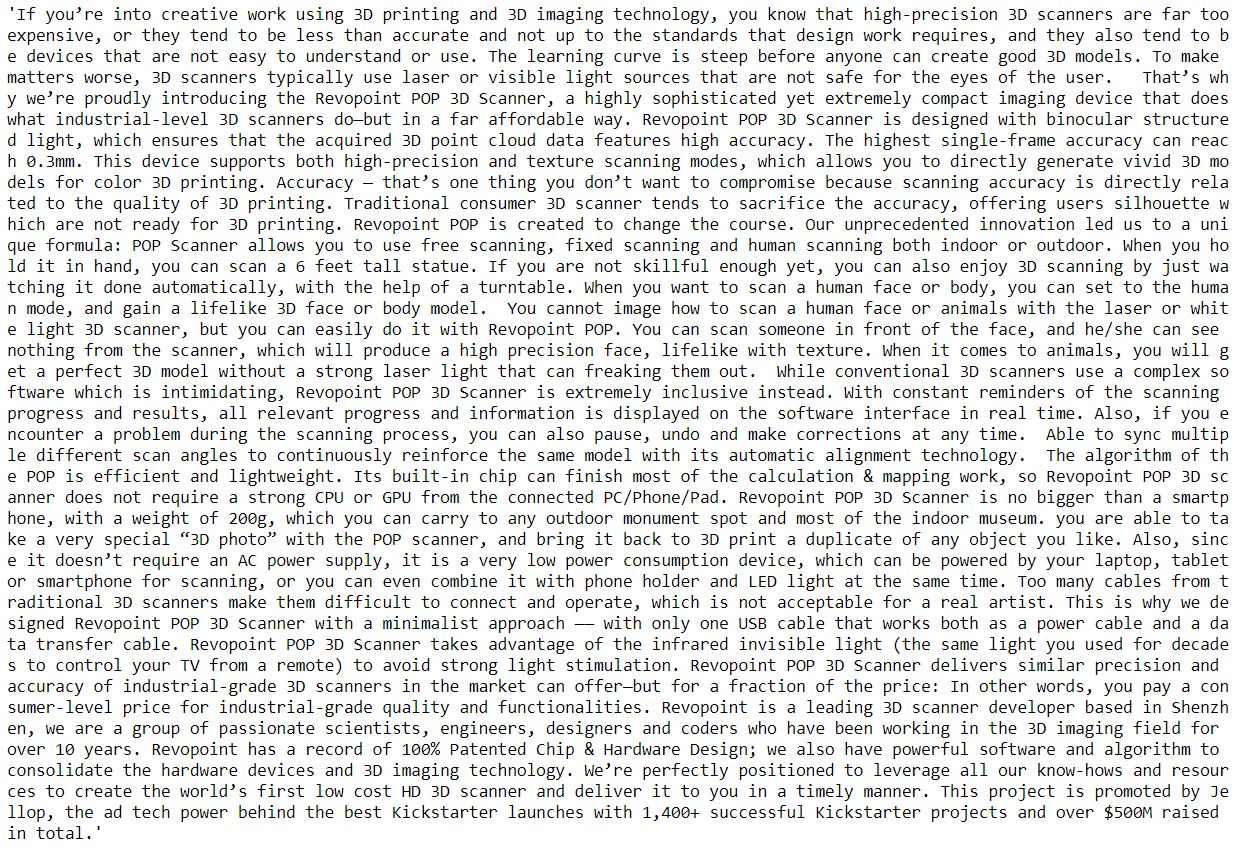
\includegraphics[width=0.95\linewidth]{4/figures/description_scraped_project.jpg}
		\caption{Descripción}
	\end{subfigure}%
	\begin{subfigure}{.50\textwidth}
		\centering
		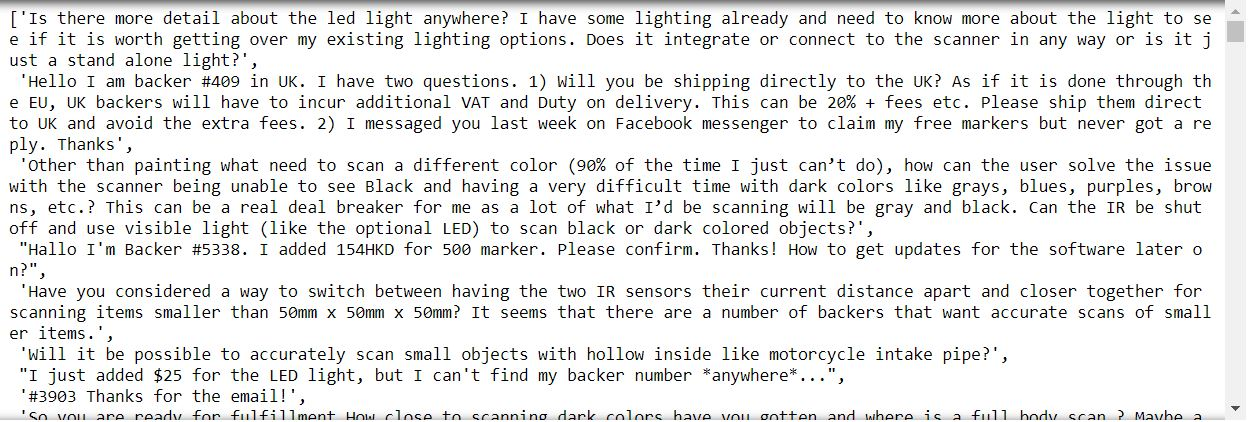
\includegraphics[width=0.95\linewidth]{4/figures/comments_scraped_project.jpg}
		\caption{Comentarios}
	\end{subfigure}
	\caption[Variables extraídas por modalidad del proyecto consultado]{Variables extraídas por modalidad del proyecto consultado.\\
		Fuente: Elaboración propia.}
	\label{4:fig40}
\end{figure}

\newpage
Esta información es pre-procesada de la misma manera que la data usada para entrenar cada modelo. A continuación, el modelo cargado The Hydra recibe los datos procesados y concatenados para realizar la predicción. Si el umbral es por lo menos 0.50, el resultado será \textbf{EXITOSO} (\textit{Successful} en inglés) como en la Figura \ref{4:fig41}.

\begin{figure}[!ht]
	\begin{center}
		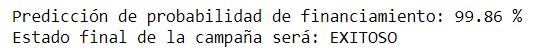
\includegraphics[width=0.70\textwidth]{4/figures/demo_project_prediction.jpg}
		\caption[Resultado de predicción de The Hydra para el proyecto consultado]{Resultado de predicción de The Hydra para el proyecto consultado.\\
			Fuente: Elaboración propia.}
		\label{4:fig41}
	\end{center}
\end{figure}